\documentclass[uplatex,dvipdfmx,a4paper,11pt]{jsarticle}

\usepackage[top=25mm,bottom=25mm,left=25mm,right=25mm]{geometry}
\usepackage{array}
\usepackage{tabularx}
\usepackage{booktabs}
\usepackage{enumitem}
\usepackage{graphicx}

\setlength{\parindent}{0pt}
\setlength{\parskip}{0.6em}

\usepackage{titlesec}
\titleformat{\section}
  {\normalfont\Large\bfseries}{\thesection.}{0.6em}{}
\titleformat{\subsection}
  {\normalfont\large\bfseries}{\thesubsection}{0.6em}{}
\titlespacing*{\section}{0pt}{1.2em}{0.6em}
\titlespacing*{\subsection}{0pt}{1.0em}{0.4em}

\newcommand{\sectionrule}{\par\medskip\noindent\rule{\linewidth}{0.6pt}\par\medskip}

\renewcommand{\labelitemi}{\textbullet}
\renewcommand{\labelitemii}{\textopenbullet}
\setlist[itemize]{leftmargin=1.6em,itemsep=0.1em,topsep=0.2em}
\setlist[enumerate]{leftmargin=2.0em,itemsep=0.1em,topsep=0.2em}

\providecommand{\textopenbullet}{\ensuremath{\circ}}

\begin{document}

{\LARGE\bfseries 作業ログ}\par\bigskip

報告者：梅澤颯太

報告日：2026年7月8日

プロジェクト名：タクトーン～IMU ジェスチャーで奏でるArduino オーケストラ～

\sectionrule

\section{進捗サマリー（要約）}

\begin{itemize}
  \item 全体進捗率：100\%
  \item マイルストーン達成状況：トランペットとホルンの音声を解析し，両楽器の音色を比較・調整できる環境を整備した．
  \item 主要成果：
    \begin{itemize}
      \item トランペットとホルンの音声サンプルを解析し，倍音構成とADSRを楽器定義JSONへ反映した．
      \item 新旧の音色合成方式を比較試聴し，両楽器のJSONを固定倍音と線形ADSR中心の構成へ調整した．
      \item 楽器プレイヤーで改善した音色を試聴できるようにし，演奏全体で確認するための通信なし輪唱チェッカーも整備した．
    \end{itemize}
  \item 課題：
    \begin{itemize}
      \item トランペットとホルンを実際の演奏に組み込み，音量，音の立ち上がり，音色のバランスを最終確認する必要がある．
      \item 追加した音響機能のうち，聴感上の効果があるパラメータを選別する必要がある．
    \end{itemize}
\end{itemize}

\subsection{ガントチャート}

\begin{figure}[htbp]
  \centering
  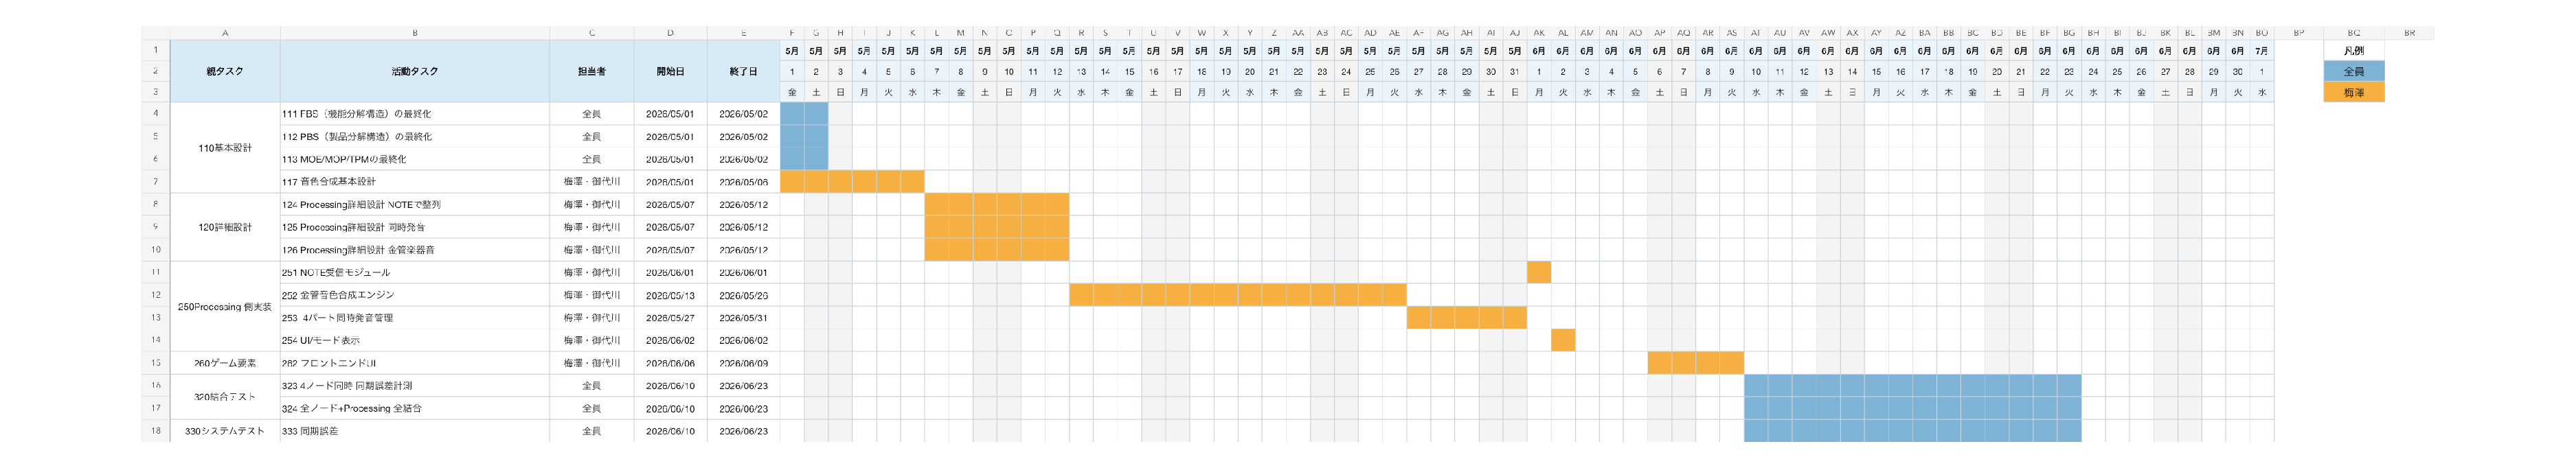
\includegraphics[width=\linewidth]{fig/ガントチャート_梅澤_全員.pdf}
  \caption{全体のガントチャート}
\end{figure}

\sectionrule

\section{作業ログ（詳細トラッキング）}

\begin{tabularx}{\linewidth}{@{}p{0.16\linewidth}p{0.12\linewidth}XX@{}}
\toprule
日付 & 作業時間 & 作業内容 & 成果・メモ \\
\midrule
2026/07/04 & 1h & トランペットとホルンの音声を解析し，音色改善用の楽器定義を作成した． & 倍音構成とADSRを抽出し，固定倍音と線形ADSRによる試聴，ホルン専用解析，音域試聴，互換JSON出力に対応した． \\
2026/07/06 & 1h & トランペットとホルンの新旧音色を比較できるようにした． & 楽器プレイヤーへ旧\texttt{test\_multi}互換再生を追加し，倍音エンベロープ，ノイズ，変調，ボディエフェクトの有無を切り替えて比較できるようにした． \\
2026/07/07 & 1h & 比較試聴の結果を基に両楽器の音色を調整した． & 改善版と旧版で聴感差が小さい機能を整理し，トランペットとホルンのJSONを固定倍音と線形ADSR中心の構成へ簡素化した． \\
2026/07/08 & 1h & 調整した音色の再生環境と全体確認用ツールを整備した． & 現行音響仕様を楽器プレイヤーへ反映してJSONの読み込みを確認した．補助作業として，金管4声とドラムを再生する通信なし輪唱チェッカーも作成した． \\
\bottomrule
\end{tabularx}

\sectionrule

\section{課題管理}

\begin{tabularx}{\linewidth}{@{}p{0.20\linewidth}Xp{0.08\linewidth}p{0.08\linewidth}Xp{0.11\linewidth}p{0.09\linewidth}@{}}
\toprule
課題 & 発生原因 & 影響度 & 優先度 & 対策 & 期限 & 状態 \\
\midrule
トランペットとホルンの最終試聴 & 単音での比較を中心に進めており，演奏全体での音量と音色のバランス確認が残っている． & 高 & 高 & 全パートを再生し，両楽器の音量と立ち上がりを調整する． & 次回作業時 & 対応中 \\
音響パラメータの選別 & 機能を追加しても旧方式との聴感差が小さい音色があった． & 中 & 中 & 新旧方式を比較試聴し，効果を確認できるパラメータだけを残す． & 最終提出前 & 対応中 \\
\bottomrule
\end{tabularx}

\sectionrule

\section{AI利用状況と検証（再現性重視）}

\subsection{利用内容}

\begin{itemize}
  \item 利用目的：トランペットとホルンの音色解析・改善，再生プログラムの実装補助，作業ログ文章の作成補助
  \item 入力（プロンプト要旨）：
    \begin{itemize}
      \item トランペットとホルンの解析結果をProcessingで再生し，新旧の合成方式を比較できるように依頼した．
      \item 比較結果を基に両楽器のJSONを調整し，演奏全体でも試聴できるように依頼した．
      \item 前週の作業ログとGit上の変更内容を基に，同じ形式で今週分を整理するよう依頼した．
    \end{itemize}
  \item 出力概要：
    \begin{itemize}
      \item トランペットとホルンの音色定義JSON，旧方式との比較機能，再生環境，作業ログを作成した．
    \end{itemize}
\end{itemize}

\sectionrule

\subsection{検証方法}

\begin{itemize}
  \item 検証手法：
    \begin{itemize}
      \item Processing CLIで各スケッチをビルドし，コンパイルエラーがないことを確認する．
      \item 楽器定義JSONの構文と実ロードを確認し，想定した音色が再生されることを確認する．
      \item 新旧方式で両楽器を比較試聴し，変更したパラメータの効果を確認する．
    \end{itemize}
  \item 検証手順：
    \begin{enumerate}
      \item \texttt{instrument\_player} と \texttt{local\_canon\_check} をビルドする．
      \item 使用するJSONを読み込み，単音再生と比較機能を確認する．
      \item 輪唱チェッカーで両楽器を含む全パートを再生し，全体の音量と音色のバランスを確認する．
    \end{enumerate}
\end{itemize}

\sectionrule

\subsection{ファクトチェック結果}

\begin{itemize}
  \item 一致点：
    \begin{itemize}
      \item トランペットとホルンの解析，JSON調整，各スケッチのビルド成功，JSONの構文確認と実ロードは作業記録と一致していた．
    \end{itemize}
  \item 不一致・疑義：
    \begin{itemize}
      \item なし．各日の作業時間は1時間，合計4時間として記録した．
    \end{itemize}
  \item 最終判断：
    \begin{itemize}
      \item 確認できた事実だけをレポート本文として採用する．
    \end{itemize}
  \item 根拠：
    \begin{itemize}
      \item 本人が提示した作業時間と，リポジトリ内の実装ファイル，ビルド結果，作業履歴メモを基に記述しているため．
    \end{itemize}
\end{itemize}

\sectionrule

\section{次回計画}

\begin{itemize}
  \item 目標：
    \begin{itemize}
      \item 改善したトランペットとホルンを演奏全体で試聴し，音量と音色のバランスを確認する．
      \item 比較結果を基に，倍音構成とADSRを最終調整する．
    \end{itemize}
  \item 達成基準：
    \begin{itemize}
      \item トランペットとホルンを聞き分けられ，演奏全体の中で両楽器の音量と音色が不自然でないこと．
      \item 最終的な倍音構成とADSRの採用理由を記録できていること．
    \end{itemize}
  \item 期限：
    \begin{itemize}
      \item 最終提出前
    \end{itemize}
\end{itemize}

\sectionrule

\section{その他}

\begin{itemize}
  \item 今週は，トランペットとホルンの音声を解析し，両楽器の音を改善することを主な作業とした．
  \item 音色を複雑にするだけでなく，旧方式と比較して効果を確認し，必要な機能を選別することを重視した．
\end{itemize}

\sectionrule

\section{付録}

無し

\end{document}
